% t. schneider

%!TEX TS-program = xelatex
%!TEX encoding = UTF-8 Unicode

\documentclass[11pt, letterpaper]{article}
\usepackage{fontspec} 
% DOCUMENT LAYOUT
\usepackage{geometry} 
\geometry{letterpaper, textwidth=5.5in, textheight=8.5in, marginparsep=7pt, marginparwidth=.6in}

% FONTS
\defaultfontfeatures{Mapping=tex-text} % converts LaTeX specials (``quotes'' --- dashes etc.) to unicode
\setromanfont[ItalicFont={Gentium Italic}]{Gentium}


% HEADINGS
\usepackage{sectsty} 
\usepackage{float}
\usepackage{graphicx} 
\graphicspath{{../images/}}
\usepackage[normalem]{ulem} 
\sectionfont{\rmfamily\mdseries\upshape\LARGE}
\subsectionfont{\rmfamily\bfseries\upshape\Large} 
\subsubsectionfont{\rmfamily\mdseries\upshape\large} 

% PDF SETUP
% ---- FILL IN HERE THE DOC TITLE AND AUTHOR
\usepackage[dvipdfm, bookmarks, colorlinks, breaklinks, pdftitle={Goby User Manual},pdfauthor={Toby Schneider}]{hyperref}  
\hypersetup{linkcolor=blue,citecolor=blue,filecolor=black,urlcolor=blue} 
\newcommand{\xmltag}[1]{{$<$\tt #1$>$}}


% DOCUMENT

\begin{document}
\begin{figure}[H]
\begin{minipage}[b]{0.55\linewidth}
\begin{LARGE}
User Manual
\end{LARGE}
\vspace{0.5em}\\
\begin{Large}
Goby Underwater Autonomy Project
\end{Large}
\vspace{0.5em}\\
\begin{footnotesize}
T. Schneider tes@mit.edu \\
Laboratory for Autonomous Marine Sensing Systems \\
MIT / WHOI Joint Program in Oceanography \& Ocean Engineering
\end{footnotesize}
\end{minipage}
\hfill
\begin{minipage}[b]{0.3\linewidth}
\begin{flushright}

\includegraphics[width=2in]{gobysoft_logo} 
\end{flushright}
\end{minipage}
\end{figure}

\vspace{0.5em}
\rule{\textwidth}{1pt}
\vspace{0.5em}

\tableofcontents

\section{Introduction}

\subsection{What is Goby?}

The Goby Underwater Autonomy Project is an autonomy architecture\footnote{or autonomy ``middleware''} tailored for marine robotics. It can be considered a direct descendant of \href{http://www.robots.ox.ac.uk/~mobile/MOOS/wiki/pmwiki.php}{the MOOS}, with inspiration from  \href{http://code.google.com/p/lcm/}{LCM}. The motivation for Goby was the desire to seamlessly integrate \href{http://gobysoft.com/doc/acomms.html}{acoustic networking} (and other low bandwidth channels found in marine robotics) into the autonomy middleware.

Goby allows you to
\begin{itemize}
\item create custom applications\footnote{synonymously: processes or binaries} (hereafter Goby applications) in C++ that can communicate with other Goby applications in a \href{http://en.wikipedia.org/wiki/Publish/subscribe}{publish/subscribe} manner using custom designed objects provided by \href{http://code.google.com/apis/protocolbuffers/}{Google Protocol Buffers}. This message passing service is mediated by the Goby Daemon (\texttt{gobyd})\footnote{the \texttt{gobyd} is a server and the Goby applications are clients}.
\item log message data using a choice of SQL backends (\href{http://www.sqlite.org/}{SQLite3} or \href{http://www.postgresql.org/}{PostgreSQL}), allowing a choice between simplicity and power. This SQL logger is seamlessly integrated with the Google Protocol Buffers messaging, and allows runtime queries.
\item log debugging output in a flexible manner to either the terminal window or a file or both, with fine-grained control over the verbosity.
\item robustly configure your Goby applications both using a text configuration file and/or command line options by writing a schema in Google Protocol Buffers and a single line of code. Gone are the days of manual command line and configuration file parsing and validity checking.
\end{itemize}

\subsection{Structure of this Manual}
This manual is designed to start slow with introductory features and then ramp up to more powerful features for advanced users. Please read as far as you wish and then as soon as possible get your feet wet. In fact, you may want to go \href{http://gobysoft.com/doc}{download and install} Goby now before reading further. If you have problems, please glance at the \href{https://answers.launchpad.net/goby}{answers} or \href{http://mailman.mit.edu/mailman/listinfo/goby}{sign up for} and email the listserver \href{mailto:goby@mit.edu}{goby@mit.edu}.

\subsection{How to get help}
The Goby community is here to support you. This is an open source project so we have limited time and resources, but you will find that many are willing to contribute their help, with the hope that you will do the same as you gain experience in this area. Please consult these resources and people, probably in this order of preference:

\begin{enumerate}
\item This user manual
\item Questions and Answers on Launchpad: \url{https://answers.launchpad.net/goby}.
\item The developers' documentation: \url{http://gobysoft.com/doc}.
\item Email the listserver (please \href{http://mailman.mit.edu/mailman/listinfo/goby}{sign up first}): \href{mailto:goby@mit.edu}{goby@mit.edu}.
\item Email the lead developer (T. Schneider): \href{mailto:tes@mit.edu}{tes@mit.edu}.
\end{enumerate}

\section{The Hello World application}

Goby is currently written entirely in C++. We hope to support more languages in the future, but C++ is a good blend of elegance and speed. While the core of Goby is based on a number of advanced C++ techniques, you only need a small amount of C++ knowledge to get started writing your own Goby application. If you are new to programming and C++, we recommend Prata's \href{http://www.amazon.com/Primer-Plus-5th-Stephen-Prata/dp/0672326973}{C++ Primer Plus}. If you are experienced in programming but new to C++, we recommend Stroustrup's \href{http://www.amazon.com/C-Programming-Language-Special/dp/0201700735}{The C++ Programming Language}. The website \url{www.cplusplus.com} is an excellent online reference.

This complete example is located in \href{http://bazaar.launchpad.net/~goby-dev/goby/trunk/files/head:/src/core/examples/ex1_hello_world}{goby/src/core/examples/ex1\_hello\_world} for your reference. It's probably a good idea to \href{http://gobysoft.com/doc}{download and install} Goby now so you can try this out for yourself.

This example involves passing a single type of message (class HelloWorldMsg) from one Goby application (\texttt{hello\_world1\_g}\footnote{you can name your applications whatever you want, but we like appending ``\_g'' to the end to indicate that this is a Goby application.}) to another (\texttt{hello\_world2\_g}). Since Goby has a star topology\footnote{all communications pass through \texttt{gobyd} and not directly from any Goby application to another}, \texttt{gobyd} will mediate this transaction.

For this example we will write two Goby applications and one Google Protocol Buffers (protobuf) message. See Fig. \ref{fig:hellow_world_structure} for the software structure of this example.

\begin{figure}
\centering
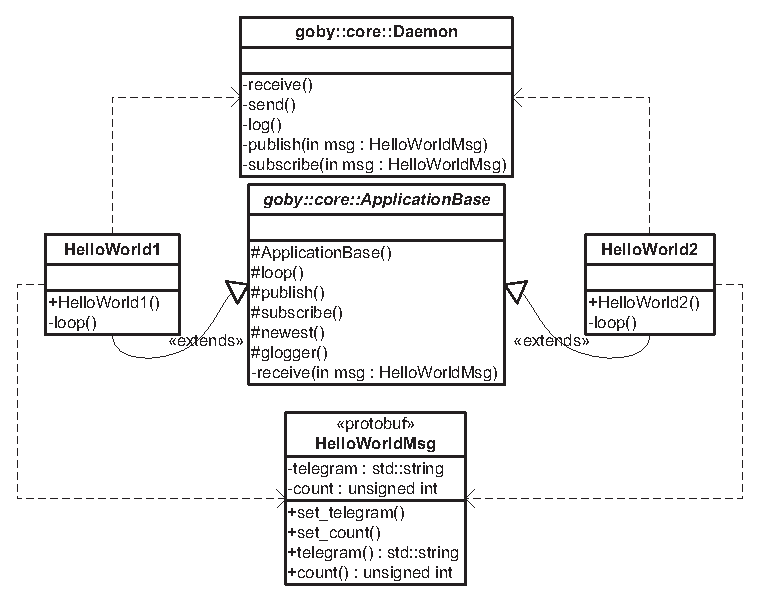
\includegraphics[scale=0.9]{hello_world_structure}
\caption{Structure diagram of the Hello World example. Solid arrows indicate generalization (inheritance) and dashed arrows indicate dependences. + is public, - is private, \# is protected.}
\label{fig:hellow_world_structure}
\end{figure}

\subsection{Meeting goby::core::ApplicationBase}

\texttt{goby::core::ApplicationBase} is the building block (base class\footnote{also called a superclass or parent class}) upon which we will make our Goby applications (which will be derived classes \footnote{also known as subclass or child class} of ApplicationBase). \texttt{ApplicationBase} provides us with a number of tools; the main ones are:

\begin{itemize}
\item a constructor \textit{ApplicationBase()} that reads the command line and configuration (we will learn about this later) and connects to \texttt{gobyd} for us.
\item a virtual method \textit{loop()} that is called at a regular frequency which is 10 Hertz by default. We will learn how to change the frequency at which \textit{loop()} is called later. 
\item a method \textit{subscribe()} which tells \texttt{gobyd} that we wish to receive all messages of this type.
\item a method \textit{newest()} which returns the newest (last received) message of a given type that we have previously called \textit{subscribe()} for. We will learn how to filter the subscriptions later.
\item a method \textit{publish()} allowing us to publish messages to \texttt{gobyd} and thereby to any subscribers of that type.
\item a method \textit{glogger()} which acts just like std::cout\footnote{\textit{glogger()} accesses goby::util::FlexOstream, a derived class of std::ostream} and lets us write to the debug (terminal window / text file) \textit{g}oby \textit{logger}.
\end{itemize}


\begin{figure}
\centering
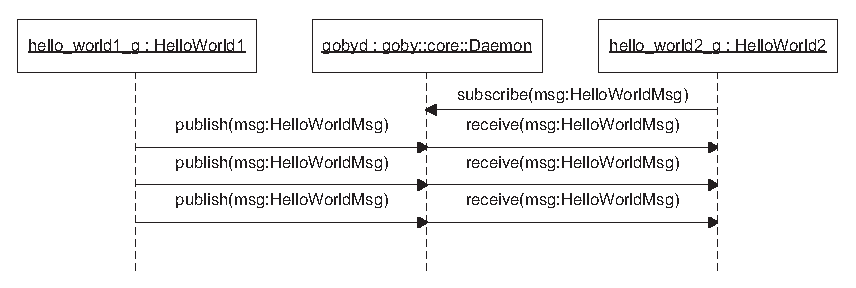
\includegraphics[scale=0.9]{hello_world_sequence}
\caption{Sequence diagram of the Hello World example.}
\label{fig:hellow_world_sequence}
\end{figure}


\subsection{Creating a simple Google Protocol Buffers Message: HelloWorldMsg}\label{sec:proto_ex}

Google Protocol Buffers (or protobuf for short) allows us to create custom classes (or structures) to for holding and transmitting data. The protobuf language is simple and looks similar to C. Protocol Buffers messages are written in .proto files and passed to the protobuf compiler (\texttt{protoc}) which generates C++ code to pass to the C++ compiler (\texttt{gcc} on Linux). Protobuf messages can contain a number of basic types (or vectors of these types) as well as nested messages. Fields are labeled as required, optional or repeated (essentially a vector). Required fields must be filled in; clearly, optional fields can be omitted. This might be a good time to read the \href{http://code.google.com/apis/protocolbuffers/docs/cpptutorial.html}{Protocol Buffers tutorial} to get a feel for the language and usage.

As you become familiar with using Protocol Buffers, the \href{http://code.google.com/apis/protocolbuffers/docs/proto.html}{language reference} will help you in creating .proto files and the \href{http://code.google.com/apis/protocolbuffers/docs/reference/cpp-generated.html}{generated code reference} will assist you in accessing the C++ classes created by the .proto files when passed through \texttt{protoc}.

For this example, we wish to send ``hello world'' (of course) so we need a string to hold our message that we will call `telegram'. Furthermore, we want to keep track of how many times we've said hello so we'll add an unsigned integer called `count'. The resulting \href{http://bazaar.launchpad.net/~goby-dev/goby/trunk/annotate/head:/src/core/examples/ex1_hello_world/hello_world.proto}{.proto file} should now be clear:
\begin{verbatim}
message HelloWorldMsg
{
  required string telegram = 1;
  required uint32 count = 2;
}
\end{verbatim}

We can set the contents of this class using calls (``mutators'' or ``setters'') like:
\begin{verbatim}
#include "hello_world.pb.h"

HelloWorldMsg msg;
msg.set_telegram("hello world");
msg.set_count(3);
\end{verbatim}

and access them using these methods (``accessors'' or ``getters''):

\begin{verbatim}
// should write "hello world: 3"
std::cout << msg.telegram() << ": " << msg.count() << std::endl;
\end{verbatim}


\subsection{Learning how to \textit{publish}: HelloWorld1}

To create a Goby application, one needs to

\begin{itemize}
\item create a derived class of \texttt{goby::core::ApplicationBase}. This is created by the following declaration:
\begin{verbatim}
class HelloWorld1 : public goby::core::ApplicationBase {};
\end{verbatim}
We also must include the goby core header (\texttt{\#include "goby/core/core.h"})
\item run the application using the \textit{goby::run()} function. Because goby::core::ApplicationBase reads our configuration (including command line options), we also pass argv and argc to \textit{run()}:
\begin{verbatim}
int main(int argc, char* argv[])
{   
    return goby::run<HelloWorld1>(argc, argv);
}
\end{verbatim}
\end{itemize}
That is all one needs to create a valid working Goby application. However, we would like our application to do a little bit more.

ApplicationBase provides a \href{http://www.cplusplus.com/doc/tutorial/polymorphism/}{virtual method} called \textit{loop()} that is called on some regular interval (it is the \textit{synchronous event} in Goby), by default 10 Hertz. By overloading \textit{loop()} in our derived class \texttt{HelloWorld1}, we can do any kind of synchronous work that needs to be done without overloading the CPU\footnote{in between calls to \textit{loop()}, ApplicationBase handles incoming subscribed messages}. In this example, we will create a simple message (of type HelloWorldMsg which we previously designed in section \ref{sec:proto_ex}) and publish it to \texttt{gobyd} and thus all subscribers (we create a subscriber in section \ref{sec:sub_ex}). 

Let's walk through each line of our \textit{loop()} method:

\begin{verbatim}
1 void loop()
2 {
3    static int i = 0;
4    HelloWorldMsg msg;
5    msg.set_telegram("hello world!");
6    msg.set_count(++i);
7    glogger() << "sending: " << msg << std::endl;
8    publish(msg);
9 }
\end{verbatim}

Line 1: \textit{loop()} takes no arguments and returns nothing (void). We declare (line 3) a static integer\footnote{static in this context means that the variable will keep its value across calls to the function \textit{loop()}.} to keep track of how many times we have looped and thus print an increasing integer value. Then we create a HelloWorldMsg called msg (line 4) and set the values of its fields (lines 5 and 6). We then publish a human debugging log message using \textit{glogger()} (just like std::cout or other std::ostreams), which will be put to the terminal window in verbose mode\footnote{goby provides operator<< for google::protobuf::Message objects as a wrapper for google::protobuf::Message::DebugString()}. Finally, we publish our message (line 8).


\subsection{Learning how to \textit{subscribe}: HelloWorld2} \label{sec:sub_ex}

Now that our hello\_world1\_g application is publishing a message, we would like to create an application that subscribes for it. To subscribe for a message, we typically provide two things:
\begin{itemize}
\item The type of the message we want to subscribe for (e.g. HelloWorldMsg).
\item A method or function that should be called when we receive that type (a callback).
\end{itemize}

Subscriptions typically take place in the constructor (here, HelloWorld2::HelloWorld2()), but can happen at any time as needed (within \textit{loop()}, for example). You subscribe for a type once, and then you will continue to receive all other applications' publishes to that type.

We subscribe for a type using a call to \textit{subscribe()} that looks like this:
\begin{verbatim}
subscribe<HelloWorldMsg>(&HelloWorld2::receive_msg, this);
\end{verbatim}

While a bit complicated at first, this call should make sense shortly. It reads ``\textit{subscribe} for all messages of type \textit{HelloWorldMsg} and when you receive one, call the method \textit{HelloWorld2::receive\_msg} which is a member of \textit{this} class (HelloWorld2).''\footnote{You can call a member function (method) of another class by passing the pointer to the desired class instantiation instead of \textit{this}. Alternatively, you can call a non-class function by just giving its pointer, e.g. subscribe(\&receive\_msg).}. The method provided as a callback (here \textit{receive\_msg()}) must have the signature
\begin{verbatim}
void func(const ProtoBufMessage&); 
\end{verbatim}
where ProtoBufMessage is the type subscribed for (here, HelloWorldMsg). \textit{receive\_msg()} has that signature
\begin{verbatim}
void HelloWorld2::receive_msg(const HelloWorldMsg& msg);
\end{verbatim}
and thus is a valid callback for this subscription. \textit{receive\_msg()} will be called immediately (an \textit{asynchronous} event) upon receipt of a message of type HelloWorldMsg unless
\begin{itemize}
\item \textit{loop()} is in the process of being called or
\item another message callback is in the process of being called.
\end{itemize}
In these cases, \textit{receive\_msg()} is called as soon as the blocking method returns. Inside of \textit{receive\_msg()} we simply post the message to the debug log:

\begin{verbatim}
void receive_msg(const HelloWorldMsg& msg)
{
   glogger() << "received: " << msg << std::endl;
}
\end{verbatim}

\subsection{Compiling our applications using CMake}

\href{http://www.cmake.org/}{CMake}, while still lacking in documentation, is probably the easiest way to build software these days, especially for cross platform support. I will briefly walk through building a Goby application using CMake within the larger Goby project configuration. If you look at the \texttt{CMakeLists.txt} file in \href{http://bazaar.launchpad.net/~goby-dev/goby/trunk/annotate/head:/src/core/examples/ex1_hello_world/CMakeLists.txt}{goby/src/core/examples/ex\_hello\_world/CMakeLists.txt}, you can see the steps needed to add our new applications to the project:

\begin{verbatim}
1 protobuf_generate_cpp(PROTO_SRCS PROTO_HDRS hello_world.proto)
2 add_executable(hello_world1_g hello_world1.cpp ${PROTO_SRCS} ${PROTO_HDRS})
3 target_link_libraries(hello_world1_g goby_core)
\end{verbatim}

Line 1 tells CMake to add "hello\_world.proto" to the files needed to be pre-compiled by the Google Protocol Buffers compiler \texttt{protoc}. protobuf\_generate\_cpp is provided by the CMake module \href{http://bazaar.launchpad.net/~goby-dev/goby/trunk/annotate/head:/cmake_modules/FindProtobufGoby.cmake}{goby/cmake\_modules/FindProtobufGoby.cmake}. Line 2 adds our application \texttt{hello\_world1\_g} to the list to be compiled by the C++ compiler, using the sources \texttt{hello\_world1.cpp} and the generated Protocol Buffers code. We append "\_g" as a convention to quickly recognize Goby applications. Line 3 links our application against the goby\_core library, which provides goby::core::ApplicationBase, our base class.

Adding \texttt{hello\_world2\_g} is directly analogous.

\subsection{Trying it all out: running from the command line}

Now, assuming you've \href{http://gobysoft.com/doc}{gone and compiled} everything, we can run the example.

You'll need three terminal windows, one for \texttt{gobyd}, and one for each of our ``hello world'' applications. You need to start \texttt{gobyd} first
\begin{verbatim}
> gobyd -p hello_auv
\end{verbatim}
I've gone ahead and named this platform ``hello\_auv''. The platform name is a unique identifier for both intra- and inter-vehicle communications in Goby. Now we can launch our two applications (order doesn't matter), with the added ``-v'' flag to indicate we want verbose terminal output:

\begin{verbatim}
> hello_world1_g -p hello_auv -v
> hello_world2_g -p hello_auv -v
\end{verbatim}

You should see \texttt{hello\_world1\_g} passing messages to \texttt{hello\_world2\_g} every 1/10th second.

\end{document}

